\documentclass[11pt,letterpaper,twoside]{article}
\usepackage[english]{babel}
\usepackage{amssymb,amsmath}
\usepackage{fancyhdr}
\usepackage{graphicx}

 \oddsidemargin  0in \evensidemargin 0in
 \topmargin   -0.25in \headheight 0.25in \headsep 0.25in
 \textwidth   6.5in \textheight 8.75in \marginparsep 0pt \marginparwidth 0pt
 \parskip 1ex  \parindent 0ex \footskip 20pt

\newfont{\bssten}{cmssbx10}
\newfont{\bssnine}{cmssbx10 scaled 900}

%%%%%%%%%%%%%%%%%%%%%%%
\newcommand{\whatizit}{Lecture 9: Introduction to Probability}
%%%%%%%%%%%%%%%%%%%%%%%


\pagestyle{fancy}  
\fancyhead{\bssnine STOR 155,  \whatizit}
\fancyhead[RE]{} \fancyhead[LO]{}
\fancyhead[LE]{\bssnine \thepage} \fancyhead[RO]{\bssnine \thepage}
\lfoot{} \cfoot{} \rfoot{}   


\newcommand{\var}{\mathrm{Var}}



\begin{document}



\thispagestyle{empty} \vspace*{-0.75in}

{\bssten STOR 155: Introduction to Data Models and Inference \hfill May 28, 2024 \\
Prof. Will Lassiter  \hfill Page 1 of \pageref{totalpag}}
\vspace{10pt}
\begin{center} {{\Large \bf \whatizit}} \end{center}

{\bf First Examples and Terminology} \vspace{6pt}

A {\bf random phenomenon} is ... \vspace{60pt}

Examples of random phenomena \vspace{150pt}

Example: Rolling a 6-sided die:

\begin{center}
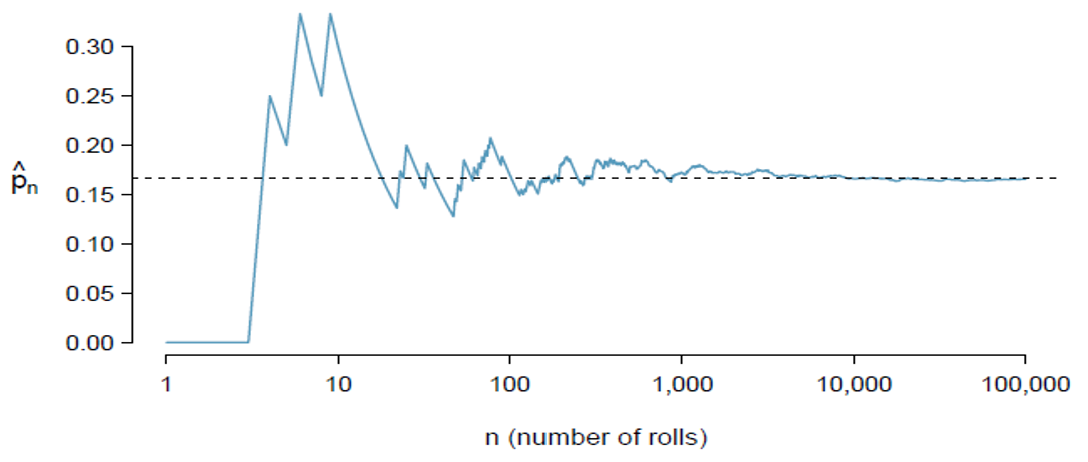
\includegraphics[scale=1]{images/longterm.png}
\end{center}

Let $\hat{p}_n=$ \vspace{30pt}

Let $p=$ \vspace{30pt}

The tendency for $\hat{p}_n$ to approach $p$ as $n$ increases is ...

\newpage

Another example: Playing cards

\begin{center}
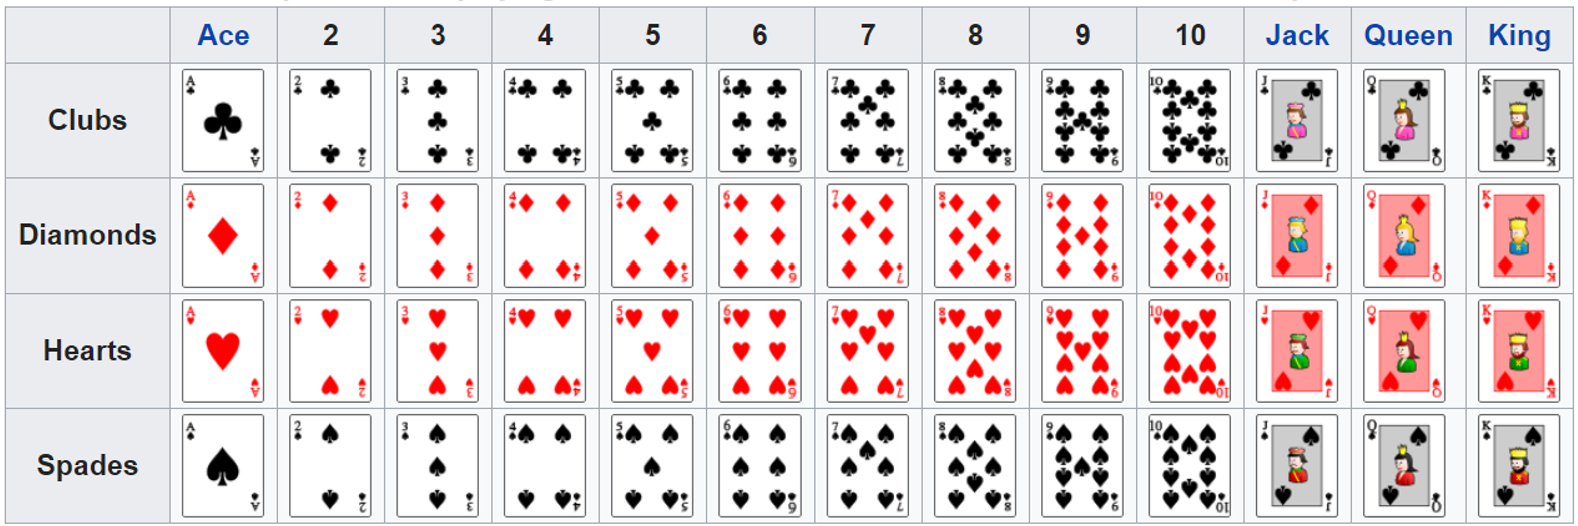
\includegraphics[scale=0.75]{images/cards.png}
\end{center}

Random phenomenon: \vspace{40pt}

Event of interest: \vspace{40pt}

Two ways to consider probability of this event:

\begin{itemize}

\item {\bf Empirically} \vspace{120pt}

\item {\bf Theoretically}

\end{itemize}

\newpage

Building a {\bf probability distribution}:

\begin{enumerate}

\item Describe random phenomenon \vspace{20pt}

\item Describe {\bf sample space} \vspace{20pt}

\item Assign a {\bf probability} to each outcome in the sample space \vspace{20pt}

\end{enumerate}

Random phenomenon: Flip a fair coin 3 times and note the outcomes (H or T) in order 

\begin{itemize}

\item Sample space: \vspace{60pt}

\item Probabilities: \vspace{40pt}

\end{itemize}

An {\bf event} is ... \vspace{60pt}

Back to coin flip example: \vspace{80pt}

Probability of this event?

\newpage

Venn diagram representation:

\begin{center}
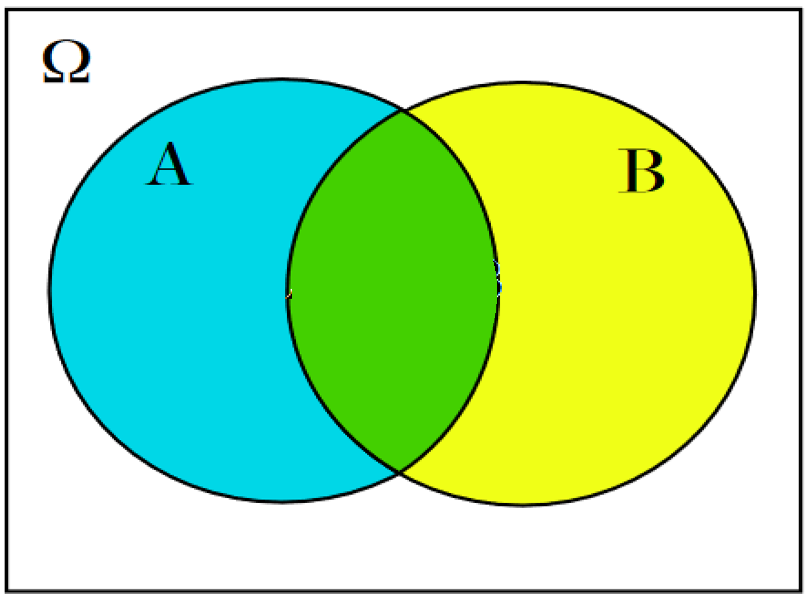
\includegraphics[scale=0.5]{images/venn.png}
\end{center}

Event operators:

\begin{itemize}

\item {\bf and} \vspace{100pt}

\item {\bf or}\vspace{100pt}

\item {\bf complement}

\end{itemize}

\newpage

Random phenomenon: Toss a coin 10 times and record the number of times it lands on heads \vspace{10pt}

Sample space? \vspace{30pt}

Let's define some events: \vspace{80pt}

Describe the event ($A$ or $B$) \vspace{60pt}

Describe the event ($A$ and $B$) \vspace{60pt}

Are $A$ and $C$ disjoint events? \vspace{30pt}

Describe the event $A^c$ \vspace{60pt}

{\bf Four basic rules for event probabilities}:

\begin{enumerate}

\item For any event $A$,\quad $0\leq P(A)\leq 1$. \vspace{10pt}

\item $P(\Omega)=1$. \vspace{10pt}

\item If events $A$ and $B$ are disjoint, then $P(A\text{ or }B)=P(A)+P(B)$. \vspace{10pt}

\item For any event $A$,\quad $P(A^c)=1-P(A)$.

\end{enumerate}

\newpage

Example: Benford's Law \vspace{6pt}

Random phenomenon: Take a table of financial, demographic, or similar numerical data, randomly select one observation, and check its first digit. \vspace{10pt}

Sample space? \vspace{20pt}  

{\em Benford's Law} postulates that all digits are not equally likely!

\begin{center}
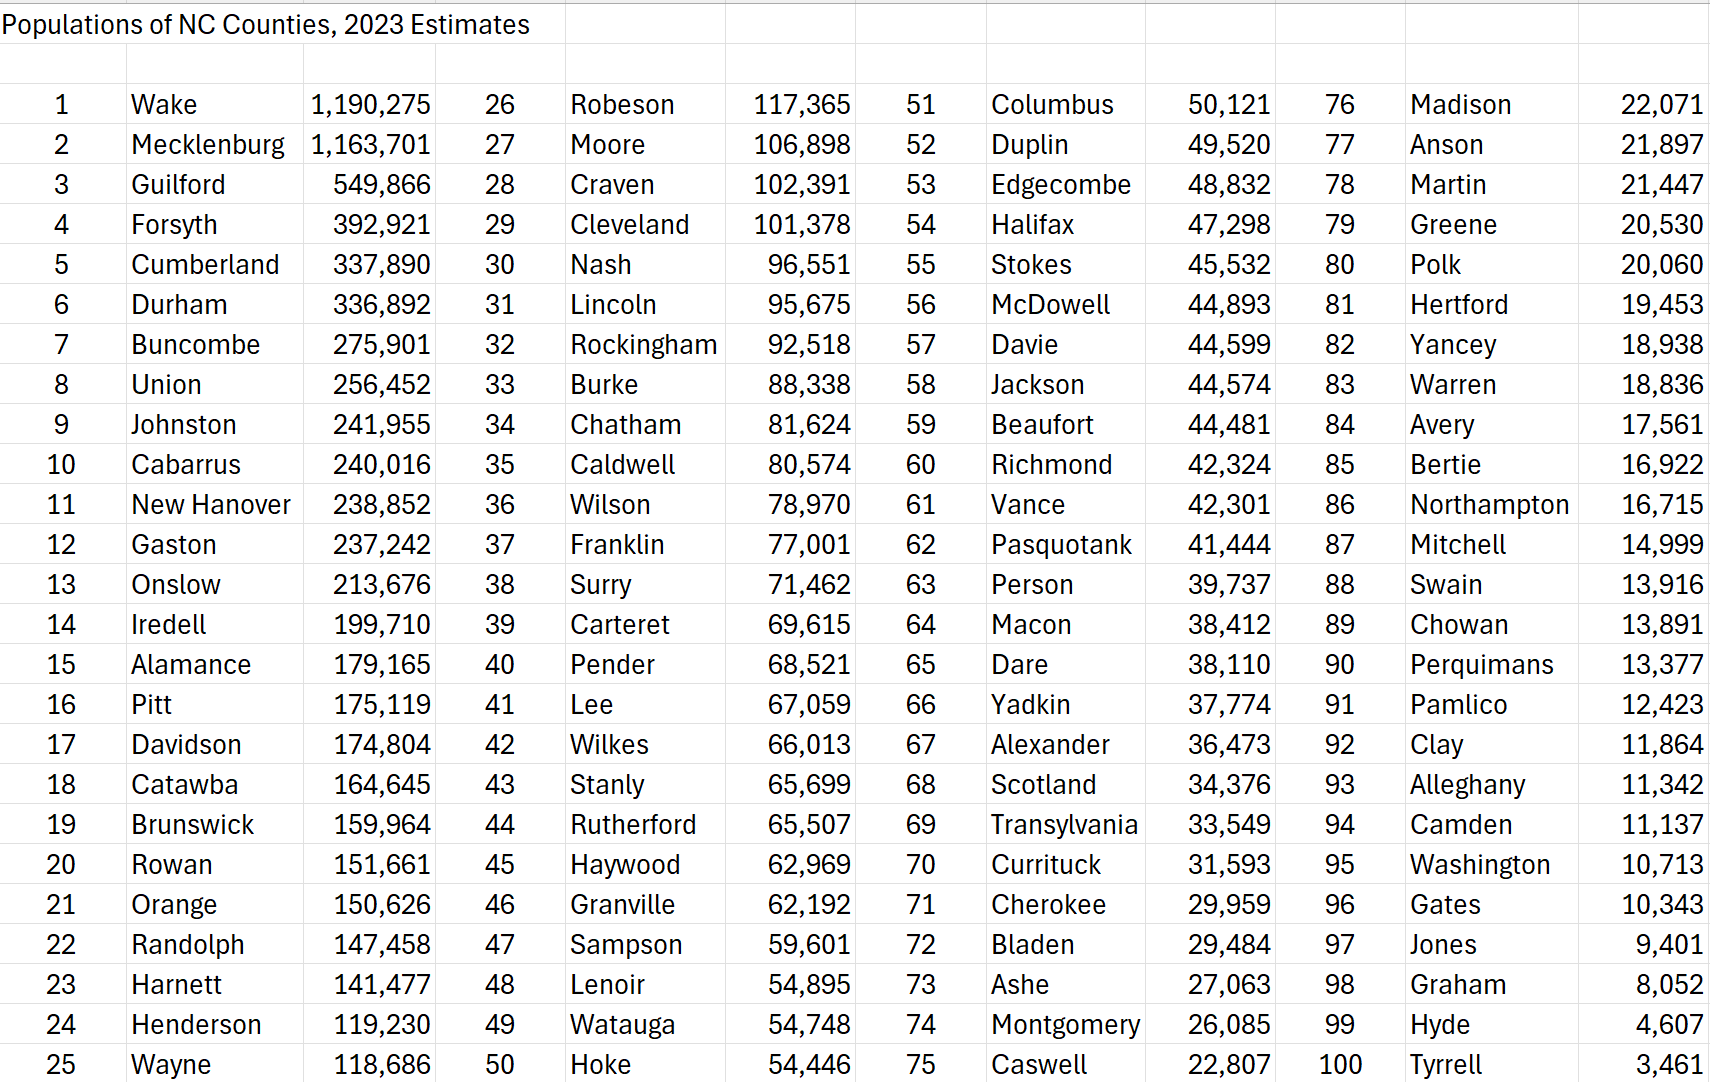
\includegraphics[scale=0.5]{images/counties.png}
\end{center}

\begin{center}
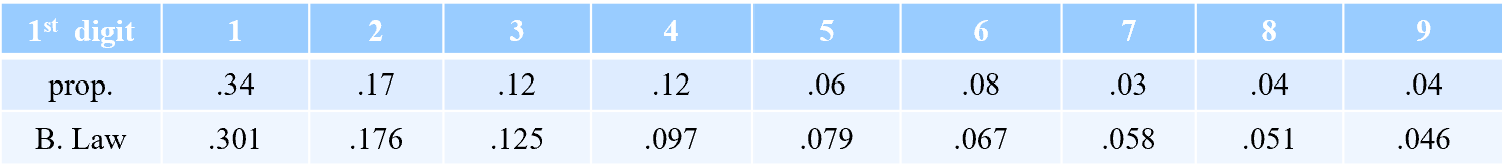
\includegraphics[scale=0.75]{images/benford2.png}
\end{center}

Let $X$ represent the first digit of a number picked at random from a data set that follows Benford's Law exactly.  Calculate:

\begin{itemize}

\item $P(X=1\text{ or }X=2)$ \vspace{30pt}

\item $P(X>2)$ \vspace{30pt}

\item $P(X\text{ is even})$ \vspace{30pt}

\item $P(X=1\text{ or }X\text{ is even})$

\end{itemize}
 
\newpage

Random phenomenon: Roll three fair, six-sided dice and count the number of 6's that come up, represent this count with $X$ \vspace{10pt}

Sample space? \vspace{20pt}

Probability distribution:
\begin{center}
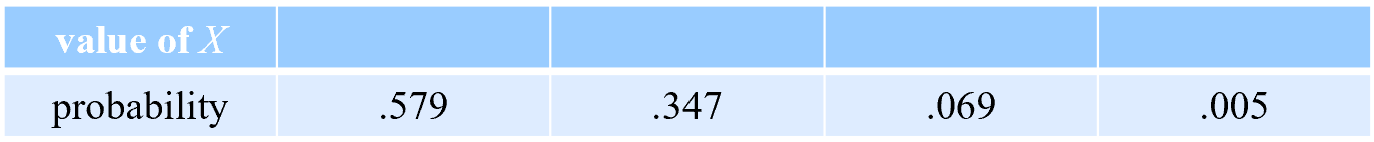
\includegraphics[scale=0.75]{images/dice.png}
\end{center}

Calculate:
\begin{itemize}

\item $P(X=2\text{ or }X=3)$ \vspace{30pt}

\item $P(X\neq 0)$ \vspace{90pt}

\end{itemize}

Random phenomenon: Take a SRS of size 2 from a group of 5 people: Alice, Bob, Cindy, Dave, Eva \vspace{10pt}

Sample space? \vspace{60pt}

Probability distribution: \vspace{40pt}

Calculate:
\begin{itemize}

\item $P(\text{Bob is chosen but Cindy is not})$ \vspace{30pt}

\item $P(\text{Bob or Cindy is chosen})$

\end{itemize}

\newpage

Random phenomenon: Draw the top card from a well-shuffled standard deck 

\begin{center}
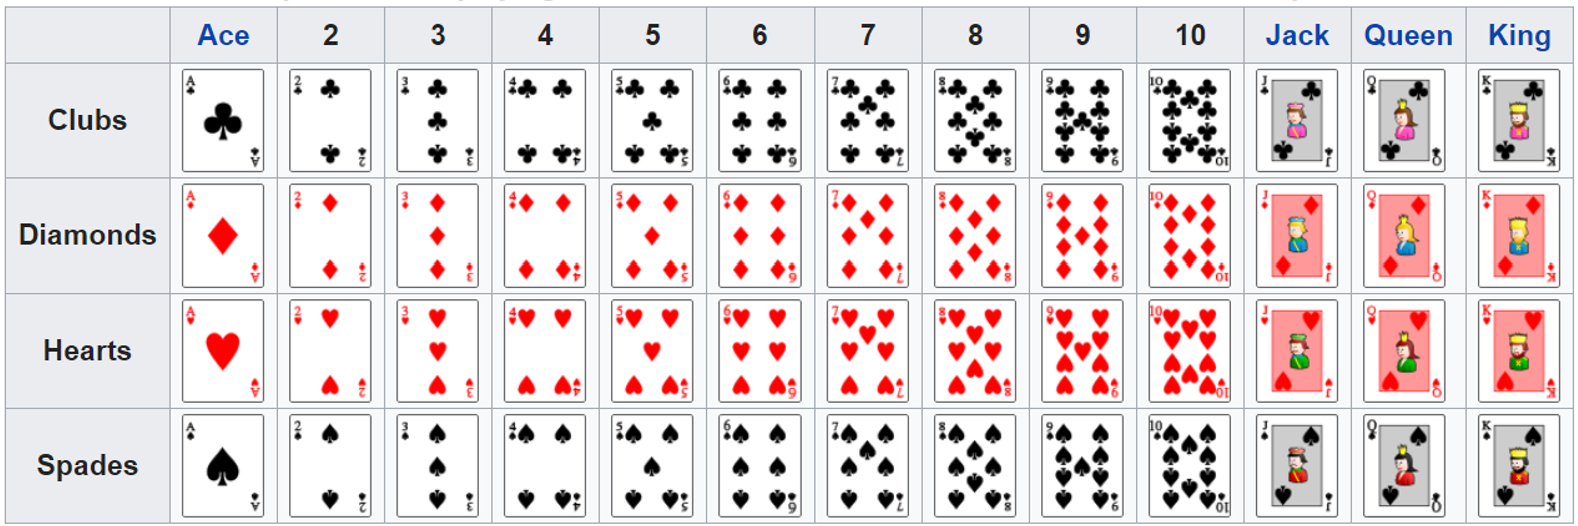
\includegraphics[scale=0.75]{images/cards.png}
\end{center}

Event $A$: The card drawn is a diamond.

Event $B$: The card drawn is a face card. \vspace{10pt}

$P(A)=$ \hspace{200pt} $P(B)=$ \vspace{20pt}

$P(A\text{ or }B)=$ \vspace{100pt}

A more general rule for calculating $P(A\text{ or }B)$:

\newpage

{\bf Independence and the Multiplication Rule} \vspace{6pt}

Two events $A$ and $B$ are {\bf independent} if ... \vspace{60pt}

Examples: \vspace{120pt}

{\bf Multiplication rule} for independent events: \vspace{60pt}

Random phenomenon: Roll a fair six-sided die twice, record both roll outcomes \vspace{10pt}

Event $A$: The first roll comes up 6. \vspace{10pt}

Event $B$: The second roll comes up 6. \vspace{10pt}

Are $A$ and $B$ independent? \vspace{50pt}

Are $A$ and $B$ disjoint? \vspace{50pt}

$P(A\text{ and }B)=$ \vspace{50pt}

$P(A\text{ or }B)=$

\newpage

Random phenomenon: Take SRS of size 2 from a group of 5 people: Alice, Bob, Cindy, Dave, Eva \vspace{10pt}

Recall sample space:\quad \{Alice, Bob\}\quad\{Alice, Cindy\}\quad\{Alice, Dave\}\quad\{Alice, Eva\}\quad\{Bob, Cindy\}

\hspace{113pt}\{Bob, Dave\}\quad\{Bob, Eva\}\quad\{Cindy, Dave\}\quad\{Cindy, Eva\}\quad\{Eva, Dave\} \vspace{10pt}

Event $A$: Alice is selected. \vspace{10pt}

Event $B$: Bob is selected. \vspace{10pt}

Are $A$ and $B$ independent? \vspace{50pt}

Are $A$ and $B$ disjoint? \vspace{50pt}

$P(A\text{ and }B)=$ \vspace{50pt}

Random phenomenon: Roll three fair, six-sided dice and count the number of 6's that come up, represent this count with $X$ \vspace{10pt}

Probability distribution:
\begin{center}
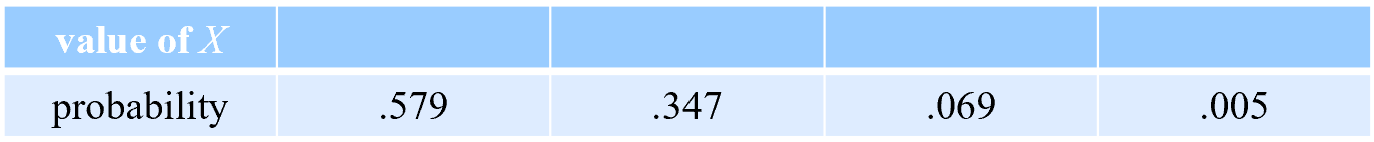
\includegraphics[scale=0.75]{images/dice.png}
\end{center}

We now know enough to get two of these probabilities!

\newpage

Random phenomenon: From a very large population in which 40\% identify as Democrats, take a SRS of size 5 and note whether or not each sampled person is a Democrat.  \vspace{10pt}

Event $A$: First person sampled is a Democrat \vspace{10pt}

Event $B$: Second person sampled is a Democrat \vspace{10pt}

Events $C$, $D$, and $E$ defined similarly.  \vspace{10pt}

Are $A$, $B$, $C$, $D$, $E$ independent? \vspace{150pt}

$P(A\text{ and }B\text{ and }C\text{ and }D\text{ and }E)\approx$ \vspace{50pt}

Random phenomenon: Sample one American at random, check their age and sex. \vspace{10pt}

Event $A$: Person is female \vspace{10pt}

Event $B$: Person is 75 years of age or older \vspace{10pt}

If 51\% of Americans are female and 6\%  of Americans are 75 or older, what is $P(A\text{ and }B)$?

\label{totalpag}
\end{document}